\documentclass{ieeeaccess}
\usepackage{cite}
\usepackage{amsmath,amssymb,amsfonts}
\usepackage{algorithmic}
\usepackage{graphicx}
\usepackage{textcomp}
\usepackage{balance}
\usepackage{booktabs}
\usepackage{array}
\usepackage{tabularx}

\usepackage{bm}
\makeatletter
\AtBeginDocument{\DeclareMathVersion{bold}
\SetSymbolFont{operators}{bold}{T1}{times}{b}{n}
\SetSymbolFont{NewLetters}{bold}{T1}{times}{b}{it}
\SetMathAlphabet{\mathrm}{bold}{T1}{times}{b}{n}
\SetMathAlphabet{\mathit}{bold}{T1}{times}{b}{it}
\SetMathAlphabet{\mathbf}{bold}{T1}{times}{b}{n}
\SetMathAlphabet{\mathtt}{bold}{OT1}{pcr}{b}{n}
\SetSymbolFont{symbols}{bold}{OMS}{cmsy}{b}{n}
\renewcommand\boldmath{\@nomath\boldmath\mathversion{bold}}}
\makeatother

\def\BibTeX{{\rm B\kern-.05em{\sc i\kern-.025em b}\kern-.08em
    T\kern-.1667em\lower.7ex\hbox{E}\kern-.125emX}}

\begin{document}
\history{Date of publication xxxx 00, 2026, date of current version xxxx 00, 0000.}
\doi{10.1100/ACCESS.2026.0000000}

\title{A Multi-Agent AI Framework for Satellite-Based Amazon Wildfire Detection and Prediction with Fire Spread Modeling and Autonomous Response Coordination}

\author{\uppercase{Navaneeth Bhaskar}\authorrefmark{1} and \uppercase{Adithya S N}\authorrefmark{1}}

\address[1]{Nitte (Deemed to be University), NMAM Institute of Technology (NMAMIT), Nitte, Karnataka, India (e-mail: navbskr@gmail.com, adithyasn2487@gmail.com)}


%\tfootnote{This work was supported by [funding details].}

\markboth
{Adithya \headeretal: IEEE ACCESS}
{Adithya \headeretal: IEEE ACCESS}

\corresp{Corresponding author: Adithya S N (e-mail: adithyasn2487@gmail.com).}


\begin{abstract}
Wildfires in the Amazon are becoming more frequent and intense; however, current satellite monitoring tools can only detect fires after they start, leaving limited time to act. This paper presents a multi-agent artificial intelligence (AI) approach that combines live Sentinel-2 and Moderate Resolution Imaging Spectroradiometer (MODIS) satellite imagery, six years of fire records from the Brazilian National Institute for Space Research (INPE), and European Centre for Medium-Range Weather Forecasts Reanalysis Version 5 (ERA5) weather data to enable proactive wildfire detection and prediction, fire spread modeling, and autonomous response coordination throughout the Brazilian Amazon. The framework integrates a five-agent large language model (LLM) coordination system to bridge the gap between satellite-based wildfire intelligence and field response. A deterministic optimizer assigns response crews based on population distribution and conservation priorities, while a Commander agent interprets the deployment plan and triggers re-optimization when needed. Field agents use Dijkstra's shortest-path algorithm to assess route feasibility, and an Evaluator agent evaluates the robustness of the deployment plan and initiates re-optimization when required. The Light Gradient Boosting Machine (LightGBM) model trained on 200,000 samples achieved a receiver operating characteristic–area under the curve (ROC-AUC) of 0.9874 and an accuracy of 95.55\%, and SHapley Additive exPlanations (SHAP) identified temperature, humidity, and agricultural land cover as the dominant wildfire drivers. A Rothermel-based cellular automata (CA) model was used to simulate fire spread, and 94.1\% of the simulated burn area was correctly identified as high risk. The proposed framework demonstrates the effectiveness of multi-agent AI for large-scale wildfire management, where, with six response crews, it intercepts 54.5\% of the advancing fire front, protects 83,031,ha, and generates coordinated response plans in 35,s.
\end{abstract}

\begin{keywords}
Amazon wildfire detection, satellite remote sensing, multi-agent AI systems, fire spread prediction, LightGBM fire susceptibility, LLM agent coordination, ecological risk assessment.
\end{keywords}

\titlepgskip=-21pt

\maketitle
\section{Introduction}
\label{sec:introduction}

\PARstart{T}{he} Amazon rainforest, which stretches across nine South American countries and covers over 5.5 million km², is the world's largest tropical forest, playing an essential role in the Earth's ecological equilibrium. It captures vast quantities of $CO_2$, controls regional rainfall, and supports over 10\% of the world's biodiversity. This irreplaceable ecosystem has suffered an alarming increase in wildfire frequency and severity over the last few decades due to a combination of prolonged dry seasons, warmer temperatures, and the inexorable advance of agriculture into the forest interior. The National Institute for Space Research (INPE) of Brazil has reported tens of thousands of wildfire events annually across the Amazon rainforest, with the peak fire season occurring between August and October. The consequences of these fires include forest ecosystem degradation, displacement of indigenous peoples, and high carbon emissions. The Amazon is not only a regional issue; large-scale wildfires have global impacts on carbon budgets, hydrological cycles, biodiversity, and the people who have lived in these forests for generations. This has made the development of increasingly intelligent and proactive wildfire management systems an important research priority.

Despite significant advances in satellite remote sensing over the past two decades, the dominant operational paradigm for Amazon wildfire monitoring remains fundamentally reactive. Systems such as NASA's Fire Information for Resource Management System (FIRMS) provide near-real-time active fire detections using the Visible Infrared Imaging Radiometer Suite (VIIRS) and Moderate Resolution Imaging Spectroradiometer (MODIS) sensors. However, these systems report fires only after ignition has already occurred, providing emergency responders with little opportunity to intervene before the fire front reaches vulnerable communities, protected ecosystems, and critical infrastructure. The limitation therefore extends beyond data availability; rather, it represents an intelligence gap between what satellite observations provide and what emergency response agencies require for timely decision-making. Raw satellite observations must be transformed into actionable intelligence capable of predicting wildfire susceptibility, forecasting fire spread under changing environmental conditions, identifying threatened ecological assets, and determining whether available response crews can reach vulnerable locations before the advancing fire front. Bridging this intelligence gap requires integrating machine learning, fire spread modelling, geospatial risk assessment, and intelligent response coordination within a unified operational framework, a capability that remains largely unexplored in existing operational wildfire management systems.

The research landscape has made significant progress on individual components of this wildfire intelligence pipeline. Gradient-boosted machine learning models trained using meteorological, terrain, and vegetation datasets have demonstrated strong wildfire susceptibility prediction performance across diverse geographical regions \cite{1}, \cite{2}. Similarly, cellular automata models derived from the Rothermel rate-of-spread formulation have shown considerable success in simulating realistic wildfire propagation at fine spatial resolutions \cite{8}. Geographic information system (GIS)-based spatial analysis has further enabled quantitative assessment of ecological vulnerability across protected areas, indigenous territories, and environmentally sensitive regions \cite{7}. Nevertheless, existing studies predominantly address wildfire detection, susceptibility mapping, or fire spread forecasting as independent tasks, and none of the reported frameworks addresses the downstream coordination problem of translating wildfire predictions into actionable emergency response. Once multiple high-risk assets are simultaneously threatened by an advancing wildfire, critical questions remain regarding how limited response crews should be optimally deployed, whether planned routes remain feasible under evolving field conditions, and how response strategies should adapt when unexpected disruptions occur.

This paper proposes a multi-agent artificial intelligence (AI) framework that, to the best of our knowledge, closes the entire operational loop from live satellite data acquisition to wildfire susceptibility prediction, fire spread modelling, ecological risk assessment, and autonomous field-response coordination. The framework constructs a large-scale training dataset by integrating six years of INPE wildfire records with European Centre for Medium-Range Weather Forecasts Reanalysis Version~5 (ERA5) meteorological data and live Sentinel-2 and MODIS satellite imagery retrieved through Google Earth Engine. A leakage-audited Light Gradient Boosting Machine (LightGBM) classifier is employed to predict wildfire susceptibility from meteorological, topographical, vegetation, and land-cover features, while SHapley Additive exPlanations (SHAP) provide model interpretability by identifying the dominant environmental drivers of wildfire occurrence \cite{3}, \cite{4}. The resulting susceptibility predictions are integrated with a Rothermel-based cellular automata model to simulate wildfire propagation under dynamically changing environmental conditions. In parallel, ecological impacts are quantified across protected areas, indigenous territories, settlements, transportation networks, and river systems using composite vulnerability indices that identify threatened assets requiring priority protection. Together, these components establish the predictive foundation upon which the proposed response coordination framework is built.

The primary contribution of this work lies in a five-agent large language model (LLM) coordination system that transforms wildfire intelligence into field-actionable emergency response plans within seconds. Importantly, crew-to-asset allocation is performed entirely by a deterministic optimization engine rather than by the language models themselves. The optimizer generates deployment plans by considering asset priorities, travel feasibility, and operational constraints, while the LLM agents provide decision support, explanation, verification, and adaptive coordination. Specifically, a Commander agent interprets the optimized allocation, explains deployment decisions according to settlement population and conservation priorities, and initiates re-optimization whenever field conditions change. Field agents independently verify route feasibility using Dijkstra's shortest-path routing over the Amazon road network, evaluate travel margins relative to predicted fire arrival times, and communicate operational observations from the field. An Evaluator agent continuously audits the robustness of the deployment plan, identifies assignments with insufficient safety margins, and triggers re-optimization whenever necessary. To ensure operational reliability, all field observations are validated against the physical state of the wildfire simulation before influencing allocation decisions, while the deterministic optimizer continues to function independently even if the LLM services become unavailable.

Collectively, the proposed framework bridges the gap between satellite-based wildfire intelligence and operational emergency response by integrating Earth observation, explainable machine learning, fire spread modelling, ecological risk assessment, deterministic optimization, and multi-agent coordination within a unified decision-support system. Unlike existing approaches that terminate at wildfire detection, susceptibility mapping, or spread forecasting, the proposed framework extends predictive intelligence to practical emergency response by enabling adaptive crew deployment under dynamically evolving field conditions. Experimental evaluation demonstrates the effectiveness of the framework across both predictive and operational tasks, achieving high wildfire susceptibility prediction performance, realistic fire spread simulation, and robust multi-agent response coordination across multiple deployment scenarios. These capabilities demonstrate the potential of integrating satellite-based Earth observation with deterministic optimization and multi-agent AI to support proactive, scalable, and reliable wildfire management in the Brazilian Amazon.


\section{Related Works}

Building on the research gap identified in the previous section, considerable progress has been made in applying machine learning, remote sensing, and simulation techniques to wildfire prediction and management. Existing studies have demonstrated significant advances in wildfire susceptibility mapping, explainable artificial intelligence (XAI), fire spread simulation, and geospatial risk assessment. However, these developments have largely remained independent research directions, with relatively limited attention devoted to integrating predictive wildfire intelligence with operational emergency response. This section reviews representative studies across these domains and highlights the research gap addressed by the proposed framework.

Machine learning has emerged as one of the most effective approaches for wildfire susceptibility prediction by integrating meteorological, topographical, vegetation, and land-cover information. Xu et al.~\cite{1} proposed an LSSVM-CA framework that combines least squares support vector machines with a three-dimensional cellular automata model to simulate wildfire spread within a GIS environment. Their approach learns cellular automata transition rules directly from historical fire observations and incorporates wind direction to improve directional fire propagation. While the model successfully reproduces realistic fire spread patterns, it relies primarily on data-driven transition learning rather than explicitly modelling wildfire physics. Similarly, Abdollahi and Pradhan~\cite{2} demonstrated the importance of explainable artificial intelligence by integrating deep learning with SHAP for wildfire susceptibility prediction in Australia. Their analysis identified humidity, rainfall, elevation, slope, and vegetation moisture indices as dominant wildfire drivers while showing that XAI substantially improves the interpretability of machine learning predictions. Extending this direction, Hang et al.~\cite{3} proposed a stacked ensemble framework combining AdaBoost, Gradient Boosting Machine, XGBoost, Random Forest, and a Deep Neural Network for wildfire susceptibility mapping in the Western Himalaya. Their results showed that ensemble learning consistently achieved superior predictive performance, while SHAP and Local Interpretable Model-Agnostic Explanations (LIME) provided both global and local feature explanations. Likewise, Iban and Aksu~\cite{4} evaluated Random Forest, XGBoost, and LightGBM models for wildfire susceptibility mapping using MODIS fire observations in Türkiye. Their SHAP analysis highlighted temperature, wind speed, Normalized Difference Vegetation Index (NDVI), slope, and anthropogenic proximity as dominant contributors to wildfire occurrence. Collectively, these studies demonstrate the effectiveness of gradient-boosted learning algorithms and explainable AI for wildfire prediction, motivating the adoption of LightGBM together with SHAP and LIME within the proposed framework.

Alongside susceptibility prediction, considerable attention has been devoted to modelling wildfire propagation using both machine learning and simulation-based techniques. Rubí et al.~\cite{5} applied multiple machine learning algorithms to predict wildfire spread in the Brazilian Cerrado biome using climatic observations, satellite imagery, topographical information, and environmental variables, with AdaBoost achieving the highest prediction accuracy. Perello et al.~\cite{8} employed the PROPAGATOR cellular automata simulator to support prescribed fire planning in the Liguria region of Italy, demonstrating that cellular automata can provide practical decision-support capabilities for operational wildfire management. Although these studies successfully model wildfire dynamics, they primarily focus on predicting fire behaviour and do not extend their analyses to downstream emergency response planning or resource allocation. In contrast, the proposed framework employs a Rothermel-based cellular automata model to simulate wildfire propagation and directly integrates the predicted fire arrival information into a multi-agent coordination framework for real-time operational decision making.

Recent studies have also demonstrated the growing importance of integrating satellite remote sensing with machine learning for large-scale wildfire monitoring and prediction. Tang et al.~\cite{6} developed a machine learning-based wildfire warning system for Thailand using fire occurrence records and remotely sensed data acquired through Google Earth Engine (GEE). Among the evaluated classifiers, Extreme Gradient Boosting (XGBoost) achieved the highest predictive performance, demonstrating the effectiveness of gradient-boosted tree models for large-scale wildfire forecasting. Within the Brazilian Amazon, Luz et al.~\cite{7} proposed an unsupervised framework for wildfire susceptibility mapping by combining multitemporal Landsat-8 and MODIS imagery with anomaly detection techniques. Although the approach successfully identified wildfire-prone regions without requiring labelled data, its unsupervised formulation limited the integration of meteorological and terrain variables that strongly influence wildfire behaviour. Freitas et al.~\cite{9} further investigated wildfire susceptibility prediction within the Triunfo do Xingu Environmental Protection Area using Random Forest and XGBoost regression models, demonstrating excellent predictive performance and reinforcing the suitability of tree-based ensemble learning for Amazon wildfire applications. Complementing these studies, De Santana et al.~\cite{10} employed the Maximum Entropy (MaxEnt) model to analyse present and future wildfire dynamics across the Amazon under different socioeconomic scenarios. Their findings identified proximity to agricultural land as the dominant wildfire driver, highlighting the strong influence of anthropogenic activities on Amazon fire occurrence. Collectively, these studies demonstrate the value of combining satellite observations, environmental variables, and machine learning for regional wildfire prediction while emphasizing the importance of considering both climatic and human-induced factors.

Although the literature has achieved significant progress in wildfire susceptibility prediction, fire spread simulation, explainable artificial intelligence, and satellite-based environmental monitoring, these components are generally investigated as independent research problems. Existing frameworks typically terminate at wildfire detection, susceptibility mapping, or spread forecasting, leaving the downstream challenge of operational emergency response largely unexplored. In particular, current studies do not address how predictive wildfire intelligence can be translated into coordinated field operations involving dynamic crew allocation, route verification, adaptive replanning, and resource optimization under rapidly changing environmental conditions. Furthermore, deterministic optimization and multi-agent reasoning have rarely been integrated within a unified wildfire decision-support framework capable of supporting real-time emergency management.

The proposed framework addresses this research gap by coupling wildfire prediction with autonomous coordination of firefighting resources within a single end-to-end operational pipeline. Unlike previous studies that focus on isolated stages of the wildfire management process, the proposed approach extends predictive intelligence to practical emergency response, enabling adaptive field-response planning based on evolving wildfire behaviour and operational constraints.

\section{Methodology}

This section presents the proposed end-to-end wildfire intelligence framework, which integrates satellite-based Earth observation, machine learning, fire spread modelling, ecological risk assessment, and multi-agent response coordination into a unified operational pipeline. The framework consists of five sequential components: (i) dataset construction and feature engineering, (ii) wildfire susceptibility modelling, (iii) fire spread simulation, (iv) ecological and infrastructure risk assessment, and (v) multi-agent LLM response coordination. Fig.~\ref{fig:system} illustrates the overall architecture and information flow between these components.

Historical wildfire observations from the Brazilian National Institute for Space Research (INPE) are integrated with ERA5 meteorological reanalysis data and live satellite imagery retrieved through Google Earth Engine to construct the wildfire prediction dataset. The resulting susceptibility predictions are subsequently used by two parallel modules: a Rothermel-based cellular automata simulator for wildfire spread modelling and a GIS module for ecological and infrastructure risk assessment. The outputs of these modules are then supplied to a multi-agent coordination framework that generates operational response plans through deterministic optimization and LLM-assisted decision support.

\subsection{Dataset Construction and Feature Engineering}

The training dataset is constructed by integrating wildfire observations, meteorological variables, satellite-derived indices, terrain characteristics, and land-cover information across the Brazilian Amazon (Latitude: $-12^{\circ}$ to $+6^{\circ}$; Longitude: $-75^{\circ}$ to $-50^{\circ}$) for the period 2018--2023. Historical wildfire labels are obtained from the annual INPE fire detection records, where confirmed fire locations are assigned a binary label of \textit{fire} = 1. To avoid class imbalance, an equal number of non-fire locations are randomly sampled within the same spatial and temporal domain, producing a balanced dataset comprising 200,000 samples.

Meteorological information is extracted from ERA5, including temperature, relative humidity, precipitation, wind speed, and wind direction. Satellite-derived environmental variables are retrieved through Google Earth Engine using Sentinel-2 Surface Reflectance imagery for the NDVI and Normalized Burn Ratio (NBR), together with MODIS MOD11A2 land surface temperature (LST). Terrain variables, including elevation, slope, and aspect, are derived from the Shuttle Radar Topography Mission (SRTM), while land-cover information is obtained from MapBiomas Collection~9 and encoded into five categorical classes. A leakage audit is performed prior to model development to remove features that exhibit artificial correlations with the target labels, ensuring that only physically meaningful predictors are retained for subsequent analysis.

For operational deployment, meteorological conditions are estimated continuously across the wildfire monitoring region using inverse-distance-weighted (IDW) interpolation from 120 ERA5 anchor locations arranged over the Amazon domain. Weather variables at each prediction location are estimated using the six nearest anchor points according to

\begin{equation}
\hat{f}(x)=
\frac{\displaystyle\sum_{i=1}^{6}w_i(x)f_i}
{\displaystyle\sum_{i=1}^{6}w_i(x)},
\qquad
w_i(x)=\frac{1}{d(x,x_i)^2},
\label{eq:idw}
\end{equation}

where $f_i$ denotes the meteorological variable observed at anchor location $x_i$, and $d(x,x_i)$ represents the great-circle distance between the prediction location and the corresponding anchor point. This interpolation strategy provides spatially continuous meteorological inputs for wildfire susceptibility prediction throughout the study region.

Table~\ref{tab:dataset} summarises the complete set of predictor variables employed in this study. The feature set combines meteorological variables, satellite-derived spectral indices, terrain characteristics, land-cover information, and seasonal indicators, thereby providing a comprehensive representation of the environmental factors governing wildfire occurrence. Fig.~\ref{fig:dataset} illustrates the spatial distribution of the constructed dataset across the Brazilian Amazon.

\subsection{Fire Susceptibility Modelling and Explainability}

Wildfire susceptibility prediction is formulated as a supervised binary classification problem. Seven machine learning models are evaluated, namely Random Forest, XGBoost, LightGBM, CatBoost, TabNet, a multilayer perceptron (MLP), and a stacked ensemble model. All models are trained using an 80/20 train--test split with a fixed random seed to ensure reproducibility. The stacked ensemble combines the highest-performing base learners using logistic regression as a meta-classifier trained on out-of-fold probability estimates.

To support operational deployment, one production model is selected for generating wildfire susceptibility scores across the Amazon monitoring grid. Model interpretability is incorporated through SHAP and LIME. SHAP is employed to quantify the global contribution of individual predictor variables, whereas LIME provides local explanations for representative prediction instances. Together, these complementary explainability techniques improve the transparency of the prediction framework and facilitate interpretation of model behaviour during operational decision making. The quantitative performance comparison of the evaluated models and the resulting feature importance analyses are presented in Section~\ref{sec:results}.

\subsection{Fire Spread Simulation}

The wildfire susceptibility map generated by the prediction model is subsequently integrated with a cellular automata (CA) framework to simulate wildfire propagation under dynamic environmental conditions. The simulation is performed on a $51 \times 51$ grid with a spatial resolution of 100\,m per cell, representing a $51\,\text{km} \times 51\,\text{km}$ study domain. Each grid cell is assigned environmental attributes, including vegetation condition, land-cover type, elevation, slope, and aspect, through nearest-neighbour mapping from the constructed dataset. Meteorological conditions, including temperature, humidity, wind speed, and wind direction, are initialized from the ignition location and assumed constant throughout the simulation horizon.

Fuel availability is determined from vegetation condition using the NDVI, which is converted into a fuel moisture flammability factor $F_m \in [0,1]$. Lower NDVI values correspond to drier vegetation with higher flammability, whereas dense vegetation with high NDVI values is assigned lower ignition potential after adjustment for ambient humidity. A land-cover fuel weight $F_t$ is assigned to each MapBiomas land-cover class to represent the relative combustibility of different surface types, with water bodies treated as non-burnable barriers.

Wind influences wildfire propagation through a directional weighting function defined as

\begin{equation}
W_f(\alpha)=\frac{U}{5}\cdot w(\alpha,\theta_{\text{wind}})
\label{eq:wind}
\end{equation}

where $U$ denotes wind speed (m/s), $\alpha$ represents the direction from the current cell toward a neighbouring cell, and $w(\alpha,\theta_{\text{wind}})$ is a directional alignment multiplier determined from the angular difference between the spread direction and the prevailing wind direction.

Terrain effects are incorporated using a slope correction factor

\begin{equation}
S_f=
\begin{cases}
1+\theta_s/30, & \text{uphill}\\
\max(0.3,\;1-\theta_s/60), & \text{downhill}
\end{cases}
\label{eq:slope}
\end{equation}

where $\theta_s$ denotes the slope angle of the destination cell. Positive slopes promote uphill fire propagation, whereas downhill movement reduces the probability of spread.

The overall transition probability governing wildfire propagation between neighbouring cells is computed as

\begin{equation}
P_{\text{spread}}(r,c \rightarrow r',c')
=
F_m
\cdot
F_t
\cdot
W_f(\alpha)
\cdot
S_f,
\label{eq:spread}
\end{equation}

where the resulting probability is constrained to the interval $[0,1]$. A small stochastic perturbation is introduced during each simulation step to represent local environmental variability that cannot be explicitly modelled. Water bodies are treated as permanent firebreaks with zero propagation probability, while burning cells transition to a burned state after a predefined combustion period.

\subsection{Ecological and Infrastructure Risk Assessment}

To quantify the potential ecological and societal impacts of predicted wildfires, the simulated fire behaviour is integrated with multiple geospatial boundary layers representing environmentally and socially sensitive assets across the Brazilian Amazon. Spatial overlays are performed using protected-area boundaries obtained from the Chico Mendes Institute for Biodiversity Conservation (ICMBio), indigenous territories provided by the National Foundation of Indigenous Peoples (FUNAI), settlement locations, transportation networks, and major river systems. These spatial datasets are combined with the wildfire susceptibility predictions to generate composite vulnerability measures that support emergency response prioritization.

The Protected Area Vulnerability Index (PAVI) estimates wildfire exposure across federal conservation units by weighting the average wildfire susceptibility within each protected area according to its spatial extent:

\begin{equation}
\text{PAVI}
=
10
\sum_{i=1}^{N_{\text{PA}}}
\bar{p}_i
w_i,
\qquad
w_i
=
\frac{A_i}
{\displaystyle\sum_{j=1}^{N_{\text{PA}}}A_j},
\label{eq:pavi}
\end{equation}

where $\bar{p}_i$ denotes the mean wildfire susceptibility within protected area $i$, and $A_i$ represents its corresponding area. The same formulation is employed to compute the Indigenous Territory Risk Index (ITRI) using the mapped indigenous territory boundaries.

Potential threats to populated locations are quantified using the Settlement Threat Score (STS), defined as

\begin{equation}
\text{STS}
=
\frac{
4n_{\text{CRIT}}
+
3n_{\text{High}}
+
2n_{\text{Mod}}
+
n_{\text{Low}}
}
{n_{\text{total}}},
\label{eq:sts}
\end{equation}

where the numerator represents weighted counts of surrounding wildfire risk categories and $n_{\text{total}}$ is the total number of evaluated prediction points within the specified neighbourhood.

A broader ecological assessment is provided through the Forest Vulnerability Index (FVI), which combines wildfire susceptibility, land-cover sensitivity, protected-area status, and infrastructure proximity into a single composite indicator:

\begin{equation}
\text{FVI}_j
=
10
\left(
0.40S_j
+
0.25L_j
+
0.20P_j
+
0.15I_j
\right),
\label{eq:fvi}
\end{equation}

where $S_j$ denotes wildfire susceptibility, $L_j$ represents ecological land-cover sensitivity, $P_j$ indicates whether the location lies within a protected ecological region, and $I_j$ quantifies infrastructure proximity. Together, these complementary indices provide a comprehensive assessment of wildfire impacts on ecological resources, human settlements, and critical infrastructure, thereby supporting the prioritization of response operations within the proposed coordination framework.

\subsection{Multi-Agent LLM Fire Response Coordination}
\label{sec:coord}

The final stage of the proposed framework transforms wildfire prediction, spread simulation, and ecological risk assessment into an actionable emergency response plan through a multi-agent coordination framework. The proposed framework integrates deterministic optimization with LLM-assisted coordination to support dynamic resource allocation under evolving field conditions. Importantly, all crew-to-asset assignments are computed by a deterministic optimization engine, while the LLM agents perform interpretation, verification, and adaptive coordination. This separation ensures that operational decisions remain transparent, reproducible, and independent of the language models, while still benefiting from their reasoning and communication capabilities.

The coordination framework consists of five collaborative agents operating over a shared system state. A Commander agent receives the optimized deployment plan, explains resource allocation according to asset priority and operational constraints, and initiates replanning when significant environmental changes are reported. Three Field agents independently verify travel feasibility to their assigned interception locations using shortest-path routing over the Amazon transportation network, assess route accessibility, and communicate field observations. An Evaluator agent continuously monitors the overall deployment plan, validates field reports against the wildfire simulation, identifies vulnerable assignments, and requests re-optimization whenever operational objectives are no longer satisfied. Consequently, the framework supports continuous decision refinement while maintaining consistency between predicted wildfire behaviour and field operations.

The coordination process begins by constructing a prioritized list of threatened assets from the ecological risk assessment module. Each asset is assigned a priority weight according to its ecological and societal importance, while wildfire arrival times are obtained from the cellular automata spread simulation. Travel times between each response base and threatened asset are estimated using Dijkstra's shortest-path algorithm over the road network. The feasibility margin for assigning response crew $a_i$ to threatened asset $s_j$ is defined as

\begin{equation}
\text{margin}(a_i,s_j)=
t_{\text{fire}}(s_j)
-
\left(
t_{\text{travel}}(a_i,s_j)+15
\right),
\label{eq:margin}
\end{equation}

where $t_{\text{fire}}(s_j)$ denotes the predicted wildfire arrival time, $t_{\text{travel}}(a_i,s_j)$ is the estimated travel time, and the constant 15-minute term represents the operational deployment buffer required before suppression activities commence.

To quantify the reliability of each assignment, a confidence score is computed as

\begin{equation}
\text{conf}(a_i,s_j)
=
\frac{1}
{1+\exp(-\text{margin}/20)}
\times
\begin{cases}
0.8, & \text{off-road}\\
1.0, & \text{on-road}
\end{cases},
\label{eq:conf}
\end{equation}

where the logistic function converts the feasibility margin into a normalized confidence measure while accounting for reduced accessibility under off-road travel conditions.

The deterministic optimizer evaluates the complete feasibility matrix and computes the assignment that maximizes protection of threatened assets while satisfying travel-time constraints. The Commander agent communicates the resulting deployment strategy, after which the Field agents independently verify route feasibility and submit structured observations. These reports are subsequently grounded against the physical state of the wildfire simulation before being accepted by the coordination framework. The Evaluator agent then audits the complete deployment plan and initiates deterministic re-optimization whenever insufficient safety margins or newly identified field constraints compromise the current allocation. This iterative coordination cycle continues until a robust deployment strategy is obtained or a predefined iteration limit is reached.

The operational effectiveness of the coordination framework is evaluated using the Fire Front Interception Percentage (FIP), defined as

\begin{equation}
\text{FIP}
=
\frac{N_{\text{protected}}}
{N_{\text{threatened}}}
\times100\%,
\label{eq:fip}
\end{equation}

where $N_{\text{protected}}$ represents the number of threatened assets assigned a feasible response crew and $N_{\text{threatened}}$ denotes the total number of threatened assets identified by the wildfire prediction pipeline.

The coordination framework operates in two complementary modes. In the default \emph{Asset Protection} mode, response crews are allocated to intercept wildfire fronts threatening high-priority ecological or societal assets. When no assets are predicted to be threatened within the planning horizon, the framework automatically switches to an \emph{Early Suppression} mode, in which crews are deployed to strategically selected perimeter control points for proactive containment before the wildfire reaches critical locations. Both operational modes share the same optimization engine, coordination architecture, grounding mechanism, and verification process, differing only in the objective of the deployment strategy. This design enables the proposed framework to support both proactive wildfire suppression and adaptive protection of vulnerable assets using a unified operational decision-making architecture.


\section{Results and Discussion}
\subsection{Fire Susceptibility Classification}
\label{sec:substrate-results}

Seven machine learning classifiers were trained using the 200,000-sample wildfire dataset comprising 19 leakage-audited environmental features and evaluated on a held-out test set of 40,000 samples using an 80/20 random train--test split with a fixed seed of 42. The evaluated models include Random Forest, XGBoost, LightGBM, CatBoost, TabNet, an artificial neural network/multilayer perceptron (ANN/MLP), and a stacked ensemble. Their predictive performance is summarized in Table~\ref{tab:models} using accuracy, F1-score, and receiver operating characteristic--area under the curve (ROC-AUC). Overall, tree-based ensemble models consistently outperform neural network approaches, indicating that the heterogeneous environmental variables governing wildfire occurrence in the Amazon are more effectively represented through gradient-boosting strategies than deep neural architectures. XGBoost, LightGBM, CatBoost, and the stacked ensemble all achieve accuracies exceeding 95.4\% with ROC-AUC values above 0.987, demonstrating highly stable discrimination between wildfire and non-fire conditions.

Among the evaluated models, the stacked ensemble achieves the highest ROC-AUC of 0.9876, followed closely by LightGBM (0.9874), XGBoost (0.9874), and CatBoost (0.9872). However, the improvement of the stacked ensemble over LightGBM corresponds to only 0.0002 ROC-AUC units, which is considerably smaller than the variability typically observed across repeated cross-validation experiments. Consequently, this marginal performance gain does not justify the additional computational complexity introduced by the ensemble architecture. LightGBM provides the best compromise between predictive accuracy and computational efficiency, achieving an accuracy of 95.55\%, an F1-score of 95.54\%, and a ROC-AUC of 0.9874 while maintaining substantially lower training and inference overhead than the remaining models. This balance is particularly important for operational wildfire monitoring, where wildfire susceptibility must be estimated continuously across approximately 45,000 grid locations using near-real-time satellite observations.

The remaining models exhibit comparatively lower predictive capability. Random Forest achieves an accuracy of 95.12\% with a ROC-AUC of 0.9857, confirming the robustness of ensemble bagging approaches for wildfire susceptibility prediction. Although TabNet employs sequential attention mechanisms for feature selection, its predictive performance remains comparable to Random Forest while requiring considerably longer training time, indicating that the additional model complexity offers limited practical benefit for this application. The ANN/MLP records the lowest overall performance, achieving an accuracy of 94.36\% and a ROC-AUC of 0.9820. These observations suggest that conventional neural network architectures are less effective than tree-based ensemble methods when learning from structured environmental variables comprising meteorological, topographical, vegetation, and land-cover characteristics. Overall, the comparative evaluation demonstrates that gradient-boosted decision tree models provide the most reliable and computationally efficient solution for large-scale Amazon wildfire susceptibility prediction.

Fig.~\ref{fig:roc} presents the receiver operating characteristic (ROC) curves for three representative classifiers, namely Random Forest, XGBoost, and ANN/MLP. Both XGBoost and Random Forest maintain consistently high true-positive rates across the complete range of false-positive rates, producing nearly overlapping ROC curves and confirming their strong discriminative capability. In contrast, the ANN/MLP exhibits a noticeable decline in sensitivity within the low false-positive region ($\text{FPR}<0.05$), which represents the most critical operating range for operational wildfire early-warning systems. Maintaining high recall while minimizing false alarms is essential for proactive wildfire management because excessive false positives unnecessarily consume emergency resources, whereas missed detections may allow rapidly spreading wildfires to remain unaddressed. The superior ROC characteristics of LightGBM and XGBoost therefore further justify the selection of gradient-boosted ensemble learning as the foundation of the proposed wildfire prediction framework.

\subsection{Model Explainability (SHAP and LIME)}
\label{sec:xai-results}

To improve the transparency of the wildfire susceptibility model, XAI techniques were employed to quantify both global feature importance and local prediction behaviour. SHAP values were computed using TreeExplainer on a randomly selected subset of 5,000 test samples. XGBoost was selected for SHAP analysis because its tree structure is directly supported by the exact TreeExplainer algorithm, enabling exact computation of Shapley values. Complementary LIME explanations were subsequently applied to representative prediction instances in order to verify whether local feature contributions were consistent with the global explanations obtained from SHAP.

The SHAP summary plot shown in Fig.~\ref{fig:shap} reveals that temperature is the dominant predictor of wildfire susceptibility, followed by relative humidity and agricultural land cover. Specifically, the mean absolute SHAP values for temperature (2.696) and humidity (1.348) together account for more than 60\% of the overall feature contribution, indicating that short-term meteorological conditions exert substantially greater influence on wildfire occurrence than static environmental variables. Positive SHAP values associated with increasing temperature consistently shift model predictions toward wildfire occurrence, whereas increasing humidity produces an opposing effect by reducing predicted wildfire probability. Agricultural land cover exhibits an almost exclusively positive contribution to wildfire susceptibility, reflecting the widespread use of controlled burning and land-clearing practices throughout the Amazon Arc of Deforestation. In contrast, forest land cover contributes predominantly negative SHAP values, indicating that intact forest ecosystems generally provide lower wildfire susceptibility under comparable meteorological conditions. These findings are physically consistent with the known environmental drivers of Amazon wildfires and demonstrate that the prediction model has learned meaningful relationships rather than spurious statistical correlations.

Additional insights are provided by the SHAP dependence plots shown in Fig.~\ref{fig:shap_dep}. The temperature dependence plot exhibits a pronounced nonlinear threshold, with SHAP contributions remaining close to zero below approximately 28\,°C before increasing rapidly between 30\,°C and 36\,°C. This behaviour indicates that wildfire susceptibility increases sharply once high-temperature conditions characteristic of the Amazon dry season are reached. Colour-coding by month further reveals that the largest SHAP contributions are concentrated during August, September, and October, corresponding to the peak wildfire season across the Brazilian Amazon. LIME explanations generated for representative high-risk, low-risk, and misclassified instances closely agree with the global SHAP analysis, identifying the same dominant environmental variables at the individual prediction level. The strong agreement between SHAP and LIME demonstrates that both global model behaviour and local decision boundaries remain consistent, thereby increasing confidence in the interpretability and operational reliability of the proposed wildfire susceptibility model. Together, these explainability analyses confirm that the model not only achieves high predictive performance but also bases its decisions on physically meaningful environmental processes governing wildfire occurrence.

\subsection{Fire Spread Simulation}
\label{sec:spread-results}

Following wildfire susceptibility prediction, the proposed Rothermel-based CA model was employed to simulate wildfire propagation under the prevailing environmental conditions. The simulation was automatically initialized at the highest-probability grid cell identified by the LightGBM susceptibility model, corresponding to the location ($-8.642^{\circ}$, $-63.354^{\circ}$) in the municipality of Candeias do Jamari, Rondônia, Brazil. Meteorological conditions retrieved from the live ERA5 dataset at the ignition point included a temperature of 36.3\,°C, relative humidity of 26.5\%, wind speed of 2.19\,m/s with a southeasterly wind direction (126.8°), agricultural land cover, and the month of August, all of which are highly favourable for wildfire ignition and rapid propagation. These conditions provided a realistic operational scenario for evaluating the proposed spread simulation framework.

Fig.~\ref{fig:spread} illustrates the simulated wildfire progression over a 12-hour period superimposed on the corresponding satellite imagery. The burned area is divided into four temporal propagation zones, namely Immediate (0--3\,h), Rapid (3--6\,h), Extended (6--9\,h), and Outer (9--12\,h), allowing the temporal evolution of the fire front to be clearly visualized. The ignition location is indicated by the central marker, while the predicted spread direction closely follows the prevailing northwesterly trajectory expected from the observed southeasterly wind conditions. Throughout the simulation, wildfire propagation remained strongly influenced by the interaction of fuel availability, terrain slope, vegetation characteristics, and wind direction incorporated within the Rothermel-CA transition model. The final simulated burn footprint covered 563\,ha over 24 simulation steps, corresponding to a maximum spread rate of 0.215\,km/h. Visual comparison with the underlying satellite imagery further indicates that wildfire propagation remained largely confined to agricultural and previously disturbed land-cover regions, demonstrating the physical consistency of the simulation with observed landscape characteristics.

The temporal evolution of the simulated wildfire is further illustrated in Fig.~\ref{fig:burn_growth}, which presents the cumulative burn area throughout the 12-hour simulation period. Burned area increased from 28\,ha after the first three hours to 100\,ha after six hours, before accelerating to 284\,ha at nine hours and finally reaching 563\,ha after twelve hours. This nonlinear growth pattern reflects the intrinsic behaviour of cellular automata wildfire models, where the expanding fire perimeter continuously increases the number of simultaneously burning cells, producing progressively larger burned areas during subsequent simulation steps. Such behaviour closely resembles the accelerating spread commonly observed during large wildfire events and demonstrates the capability of the proposed simulation framework to capture realistic fire dynamics rather than simple linear expansion.

An important validation of the overall wildfire intelligence pipeline is obtained by comparing the susceptibility predictions with the independently simulated burn footprint. Approximately 94.1\% of the final burned area was previously classified as either High or Very High wildfire susceptibility by the LightGBM prediction model before the spread simulation was executed. This strong spatial agreement indicates that the machine learning classifier and the cellular automata model independently identify nearly identical high-risk regions despite relying on fundamentally different modelling principles. Whereas the susceptibility model estimates the probability of wildfire occurrence from environmental conditions, the cellular automata model simulates subsequent wildfire propagation using rule-based spread mechanisms. The close correspondence between these independent components provides strong evidence that the proposed framework captures the dominant environmental processes governing wildfire occurrence and propagation across the Brazilian Amazon.

\subsection{Ecological and Infrastructure Risk Assessment}
\label{sec:eco-results}

Following wildfire spread simulation, the predicted fire footprint was integrated with multiple GIS layers to evaluate the potential impacts on ecologically sensitive regions, indigenous territories, settlements, and transportation infrastructure. Rather than simply identifying areas with elevated wildfire probability, the proposed framework translates wildfire predictions into actionable spatial risk indicators that support emergency response planning and resource prioritization. The resulting ecological risk assessment therefore represents an essential bridge between wildfire prediction and operational decision making.

The calculated PAVI of 1.3838 and ITRI of 1.1318 indicate moderate wildfire exposure across federally protected conservation areas and indigenous territories under the prevailing environmental conditions. Although these basin-wide averages suggest moderate overall vulnerability, spatial analysis reveals substantial regional variation, with southern portions of the Brazilian Amazon exhibiting considerably higher wildfire exposure than northern forested regions. This spatial variability reflects the combined influence of climatic conditions, land-cover characteristics, and anthropogenic activities, emphasizing the importance of geographically targeted wildfire mitigation strategies rather than uniform resource deployment across the entire study region.

Risk assessment at the community level is provided through the STS, which achieved a basin-wide value of 1.5846. Several settlements, including Porto Velho (risk$_{10km}=0.981$) and Xinguara (0.974), exhibited particularly high wildfire exposure due to their proximity to regions of elevated wildfire susceptibility. These findings demonstrate that the proposed framework not only predicts wildfire occurrence but also identifies communities requiring immediate operational attention before wildfire impacts become severe. Such location-specific information enables emergency responders to prioritize evacuation planning, resource allocation, and preventive suppression activities according to the relative vulnerability of individual settlements.

The FVI provides a broader assessment of wildfire impacts by integrating wildfire susceptibility, ecological sensitivity, protected-area status, and infrastructure proximity into a single composite indicator. The mean FVI value of 3.2641 indicates moderate-to-high wildfire vulnerability across the Brazilian Amazon during the evaluated period. Among the 45,000 analysed grid cells, 22 were classified as CRITICAL, 2,455 as HIGH, 15,817 as MODERATE, 12,623 as LOW, and 14,083 as MINIMAL. The concentration of CRITICAL and HIGH vulnerability cells within the southern Amazon is consistent with the well-established Arc of Deforestation, where agricultural expansion and human activities substantially increase wildfire occurrence. Unlike conventional static wildfire risk maps, these vulnerability indices are generated directly from live Sentinel-2 and MODIS satellite observations integrated with ERA5 meteorological conditions through Google Earth Engine. Consequently, the ecological risk assessment dynamically reflects current environmental conditions, enabling emergency managers to identify vulnerable ecosystems and settlements using continuously updated satellite-derived information. These risk indices subsequently serve as priority inputs for the multi-agent coordination framework, where they guide deterministic resource allocation and emergency response planning.

\subsection{Multi-Agent Coordination: Live Scalability}
\label{sec:coord-live}

The practical effectiveness of the proposed framework was evaluated through a complete end-to-end deployment of the five-agent coordination architecture with the full LLM pipeline enabled. A synthetic dry-season wildfire scenario was initialized at coordinates ($-3.0^{\circ}$, $-67.5^{\circ}$) in the western Brazilian Amazon using a fire propagation rate of 2.2\,km/h. The wildfire spread simulation identified eleven threatened assets within a 24-hour planning horizon, including settlements and ecologically sensitive regions requiring immediate intervention. The deterministic optimization engine subsequently generated response plans for three operational scenarios consisting of two, four, and six available firefighting crews, allowing the scalability of the coordination framework to be evaluated under progressively increasing resource availability.

Fig.~\ref{fig:agent_coord} presents the resulting deployment strategy superimposed on the satellite basemap. The Commander agent identifies the optimal interception strategy by assigning response crews to strategically positioned control points surrounding the advancing wildfire front. Route feasibility is independently verified by the Field agents using Dijkstra's shortest-path algorithm over the Amazon road network, while inaccessible segments are explicitly labelled as off-road where no feasible transportation route exists. The Evaluator agent continuously assesses the robustness of the deployment plan and requests deterministic re-optimization whenever route feasibility changes or newly observed field conditions invalidate the current assignment. This cooperative interaction between deterministic optimization and LLM-assisted coordination enables the framework to adapt dynamically to evolving wildfire conditions while maintaining operational consistency.

Increasing the number of available response crews substantially improves both wildfire interception capability and the total area protected. With only two deployed crews, the framework successfully protects two of the eleven threatened assets, corresponding to a FIP of 18.2\% and an estimated protected area of 21,642\,ha. Expanding the deployment to four crews doubles the number of protected assets, increasing the interception rate to 36.4\% while protecting 38,754\,ha. The largest improvement occurs when six response crews are available, where the protected area increases to 83,031\,ha and the interception rate reaches 54.5\%. Notably, the increase in protected area is proportionally greater than the increase in protected assets because the additional crews are allocated to geographically extensive protected regions with substantially larger ecological footprints. These observations demonstrate that intelligent resource allocation not only increases the number of protected assets but also maximizes the overall ecological benefit obtained from limited firefighting resources.

The operational efficiency of the proposed framework remains suitable for real-time deployment throughout all evaluated scenarios. Wall-clock execution time increases only modestly from 25.87\,s for the two-crew scenario to 35.08\,s for six deployed crews, remaining comfortably below one minute even when the complete multi-agent coordination pipeline is executed. Furthermore, the total LLM API cost remains below \$0.007 for an entire coordination cycle, indicating that large-scale deployment of the proposed framework is computationally and economically feasible. These results demonstrate that deterministic optimization combined with LLM-assisted coordination can provide adaptive wildfire response planning without introducing prohibitive computational overhead.

\subsection{Multi-Agent Coordination: Benchmark and Grounding}
\label{sec:coord-bench}

To evaluate the robustness of the coordination framework under diverse operational conditions, a comprehensive factorial benchmark consisting of 216 reproducible wildfire response scenarios was constructed by systematically varying five independent factors: weather severity, wind direction, wildfire planning horizon, road network condition, and threatened asset density. This experimental design enabled the proposed framework to be evaluated under a broad range of environmental and operational situations representative of realistic wildfire management challenges while ensuring that all scenarios remained directly comparable.

Three planning strategies sharing the same deterministic optimization engine were evaluated. The \emph{stale planner} performs optimization only once before deployment and ignores subsequent field observations. The proposed framework continuously incorporates verified field reports through iterative re-optimization, whereas the \emph{oracle planner} represents an idealized upper bound by assuming that all route disruptions are known before optimization begins. Performance was measured using realized protected priority, which evaluates the actual protection delivered after accounting for crew availability, verified route accessibility, and wildfire arrival times.

Across all benchmark scenarios, the proposed framework consistently outperformed the stale planner. Mean realized protected priority increased from 19.40 to 24.49, corresponding to an average improvement of 5.09 priority points (95\% confidence interval [4.59, 5.59]). Statistical analysis using the Wilcoxon signed-rank test confirmed that this improvement was highly significant ($p \approx 1.83\times10^{-27}$), with a rank-biserial correlation coefficient of $r_{\mathrm{rb}}=+1.00$. Among the 216 evaluated scenarios, 153 exhibited improved protection, whereas none produced degraded performance relative to the stale planner. More importantly, the proposed framework achieved statistically indistinguishable performance from the oracle planner, indicating that the iterative information-revelation mechanism successfully extracts nearly all operational value available from late-arriving field observations.

A particularly important finding is the elimination of planning optimism. Although the stale planner predicts an average protected priority of 26.31 during optimization, verification against actual field conditions reveals that only 19.40 priority units are ultimately protected, producing a planning optimism gap of 6.91 priority points. Such discrepancies are operationally significant because emergency managers may overestimate the effectiveness of available resources when relying on static deployment plans. In contrast, the proposed framework continuously validates incoming observations and immediately updates resource assignments whenever route feasibility changes, thereby eliminating this optimism gap and maintaining agreement between predicted and realized protection levels.

The robustness of the verification mechanism was further evaluated through hallucination injection experiments performed at six corruption levels ranging from $\rho=0.0$ to $\rho=0.5$. Across all 1,228 evaluated scenarios, the verification gate maintained a false acceptance rate of 0.000 while simultaneously producing no false rejections of legitimate field reports. These results demonstrate that grounding field observations against the physical wildfire simulation effectively prevents erroneous or hallucinated information from influencing operational decision making without suppressing valid observations reported by response crews.

The effectiveness of language-based report interpretation was further assessed by comparing the proposed LLM grounding mechanism with a conventional rule-based regular expression parser using 55 manually annotated field reports spanning ten operational difficulty categories. The rule-based baseline achieved an exact-match accuracy of only 0.382 because its performance deteriorated substantially when field reports deviated from predefined textual patterns. In contrast, the LLM-based grounder achieved a recall of 1.000, precision of 0.979, and exact-match accuracy of 0.982 while requiring an average processing time of only 1.233\,s per report. Integrating these grounded reports into the response planner produced an average increase of 2.94 protected priority points relative to the rule-based parser ($p \approx 1.2\times10^{-35}$), with 191 benchmark scenarios demonstrating improved operational performance and none exhibiting degraded results. These findings demonstrate that combining deterministic optimization with robust LLM-based grounding substantially improves practical wildfire response coordination while preserving operational reliability.

\subsection{Discussion}
\label{sec:discussion}

The experimental results collectively demonstrate the effectiveness of the proposed unified operational wildfire management system. The wildfire susceptibility experiments show that gradient-boosted ensemble models remain the most suitable learning paradigm for structured environmental data, with LightGBM providing the best compromise between predictive accuracy and computational efficiency. Explainability analysis further confirms that the model relies on physically meaningful environmental drivers, with temperature, humidity, and agricultural land cover emerging as the dominant contributors to wildfire occurrence. The close agreement between SHAP and LIME explanations strengthens confidence in the transparency and reliability of the proposed prediction model for operational deployment.

The strong spatial correspondence between wildfire susceptibility prediction and the independently simulated burn footprint provides important cross-validation of the proposed framework. Approximately 94.1\% of the simulated burned area was previously classified as High or Very High susceptibility, indicating that both the machine learning model and the Rothermel-based cellular automata simulation independently capture the same underlying wildfire dynamics. Furthermore, the ecological vulnerability assessment extends these predictions beyond hazard identification by translating wildfire probabilities into actionable information for protected areas, indigenous territories, settlements, and critical infrastructure. Unlike conventional susceptibility maps, these dynamically generated vulnerability indices directly support emergency response planning using continuously updated satellite observations.

The most significant contribution of this work lies in the multi-agent coordination framework, which transforms predictive wildfire intelligence into adaptive operational response plans through deterministic optimization supported by LLM-assisted coordination. The benchmark experiments demonstrate that incorporating verified field observations into iterative re-optimization substantially improves realized protection while eliminating the planning optimism commonly associated with static deployment strategies. The grounding experiments further demonstrate that LLM-based interpretation significantly outperforms rule-based parsing without compromising operational safety, while the negligible computational cost and execution time confirm the practical feasibility of real-time deployment.

Several limitations should nevertheless be acknowledged. The wildfire susceptibility model was evaluated using a class-balanced dataset, whereas operational wildfire occurrence is naturally imbalanced and should be further investigated using temporal validation and precision--recall analysis. Similarly, ecological vulnerability indices represent environmental conditions corresponding to a single meteorological snapshot and therefore vary seasonally. Finally, although the benchmark scenarios provide comprehensive evaluation across diverse operational conditions, additional validation using larger real-world emergency response datasets would further strengthen the generalizability of the proposed framework. Future work will therefore focus on incorporating temporal forecasting, dynamic suppression modelling, additional Earth observation sensors, and real-time integration with operational wildfire management agencies.


\section{Conclusion}

This paper presented a comprehensive multi-agent AI framework for proactive wildfire management in the Brazilian Amazon by integrating satellite-based wildfire susceptibility prediction, fire spread modelling, ecological risk assessment, and autonomous response coordination within a unified operational pipeline. Unlike existing studies that primarily focus on wildfire detection, susceptibility mapping, or fire spread forecasting as independent tasks, the proposed framework bridges the gap between wildfire prediction and operational emergency response through deterministic optimization supported by LLM-assisted coordination. Experimental evaluation demonstrated that the LightGBM classifier achieved a prediction accuracy of 95.55\% with a ROC-AUC of 0.9874, while explainable AI analysis identified temperature, humidity, and agricultural land cover as the dominant environmental drivers of wildfire occurrence. The Rothermel-based cellular automata model simulated a 563\,ha wildfire over a 12-hour period, with 94.1\% of the simulated burn area previously classified as High or Very High wildfire susceptibility, confirming strong agreement between the prediction and spread simulation modules. The ecological risk assessment further quantified wildfire exposure across protected areas, indigenous territories, settlements, and infrastructure using dynamically generated vulnerability indices derived from live satellite observations. The proposed multi-agent coordination framework improved the mean realized protected priority from 19.40 to 24.49 across 216 benchmark scenarios, representing a statistically significant gain of 5.09 priority points ($p \approx 1.83\times10^{-27}$), while achieving performance equivalent to the oracle planner through iterative verification and deterministic re-optimization. During live deployment, the framework increased the FIP from 18.2\% with two response crews to 54.5\% with six crews, protecting up to 83,031\,ha within 35\,s at an operational cost below \$0.007 per coordination cycle. Collectively, these results demonstrate that integrating Earth observation, explainable machine learning, fire spread simulation, deterministic optimization, and multi-agent AI provides a scalable, transparent, and reliable framework for intelligent wildfire management. Future work will focus on temporal wildfire forecasting, suppression effectiveness modelling, incorporation of additional Earth observation sensors, and validation in collaboration with operational emergency management agencies.

\section*{Acknowledgment}
The authors gratefully acknowledge the support and research facilities provided by the Nitte Centre of Excellence for Applied Artificial Intelligence and the Department of Artificial Intelligence and Data Science, NMAM Institute of Technology, Nitte (Deemed to be University), India, which made this research possible.

\begin{thebibliography}{00}

\bibitem{1}
Y.~Xu, D.~Li, H.~Ma, R.~Lin, and F.~Zhang,
``Modeling forest fire spread using machine learning-based cellular automata in a GIS environment,''
\textit{Forests}, vol.~13, no.~12, p.~1974, Nov.~2022,
doi: 10.3390/f13121974.

\bibitem{2}
A.~Abdollahi and B.~Pradhan,
``Explainable artificial intelligence (XAI) for interpreting the contributing factors feed into the wildfire susceptibility prediction model,''
\textit{Science of the Total Environment}, vol.~879, p.~163004, Jul.~2023,
doi: 10.1016/j.scitotenv.2023.163004.

\bibitem{3}
H.~T.~Hang, J.~Mallick, S.~Alqadhi, A.~A.~Bindajam, and H.~G.~Abdo,
``Exploring forest fire susceptibility and management strategies in Western Himalaya: Integrating ensemble machine learning and explainable AI for accurate prediction and comprehensive analysis,''
\textit{Environmental Technology \& Innovation}, vol.~35, p.~103655, Aug.~2024,
doi: 10.1016/j.eti.2024.103655.

\bibitem{4}
M.~C.~Iban and O.~Aksu,
``SHAP-driven explainable artificial intelligence framework for wildfire susceptibility mapping using MODIS active fire pixels: An in-depth interpretation of contributing factors in Izmir, T\"{u}rkiye,''
\textit{Remote Sensing}, vol.~16, no.~15, p.~2842, Aug.~2024,
doi: 10.3390/rs16152842.

\bibitem{5}
J.~N.~S.~Rub\'{i}, P.~H.~P.~de~Carvalho, and P.~R.~L.~Gondim,
``Application of machine learning models in the behavioral study of forest fires in the Brazilian Federal District region,''
\textit{Engineering Applications of Artificial Intelligence}, vol.~118, p.~105649, Feb.~2023,
doi: 10.1016/j.engappai.2022.105649.

\bibitem{6}
J.~Tang, M.~Weeramongkolkul, S.~Suwankesawong, K.~Saengtabtim, N.~Leelawat, and K.~Wongwailikhit,
``Toward a more resilient Thailand: Developing a machine learning-powered forest fire warning system,''
\textit{Heliyon}, vol.~10, no.~13, p.~e34021, Jul.~2024,
doi: 10.1016/j.heliyon.2024.e34021.

\bibitem{7}
A.~E.~O.~Luz, R.~G.~Negri, K.~G.~Massi, M.~Colnago, E.~A.~Silva, and W.~Casaca,
``Mapping fire susceptibility in the Brazilian Amazon forests using multitemporal remote sensing and time-varying unsupervised anomaly detection,''
\textit{Remote Sensing}, vol.~14, no.~10, p.~2429, May~2022,
doi: 10.3390/rs14102429.

\bibitem{8}
N.~Perello, A.~Trucchia, F.~Baghino, B.~S.~Asif, L.~Palmieri, N.~Rebora, and P.~Fiorucci,
``Cellular automata-based simulators for the design of prescribed fire plans: the case study of Liguria, Italy,''
\textit{Fire Ecology}, vol.~20, no.~1, p.~7, Jan.~2024,
doi: 10.1186/s42408-023-00239-7.

\bibitem{9}
K.~M.~Freitas, R.~S.~Juvanhol, C.~J.~G.~Pinheiro, and A.~A.~de~M.~Meneses,
``Prediction of forest fire susceptibility using machine learning tools in the Triunfo do Xingu Environmental Protection Area, Amazon, Brazil,''
\textit{SSRN Electronic Journal}, 2024,
doi: 10.2139/ssrn.5039001.

\bibitem{10}
M.~M.~M.~de~Santana, R.~N.~de~Vasconcelos, E.~Mariano~Neto, and W.~de~J.~S.~da~Fran\c{c}a~Rocha,
``Machine learning model reveals land use and climate's role in Amazon wildfires: Present and future scenarios,''
\textit{Fire}, vol.~7, no.~10, p.~338, Oct.~2024,
doi: 10.3390/fire7100338.

\end{thebibliography}

% -----------------------------------------------------------------------
% FIGURES AND TABLES (placed together after the references)
% -----------------------------------------------------------------------
\clearpage

\begin{figure*}[p]
  \centering
  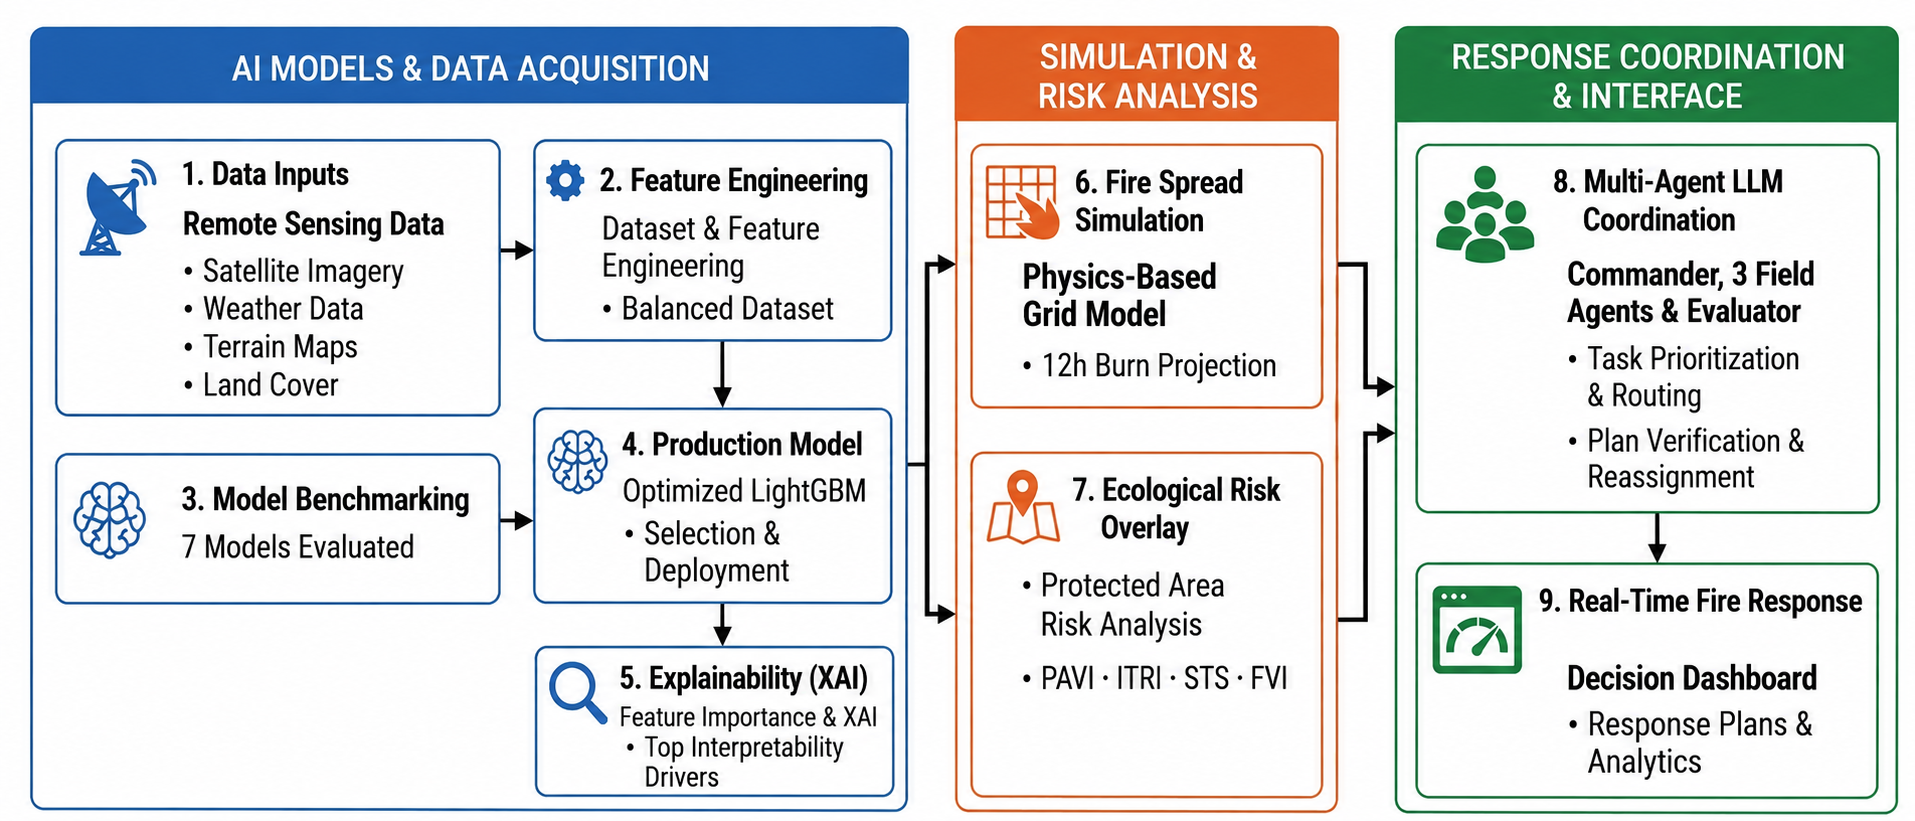
\includegraphics[width=\textwidth]{fig1_system_block_diagram.png}
  \caption{End-to-end system architecture of the proposed Amazon wildfire intelligence framework.}
  \label{fig:system}
\end{figure*}

\begin{figure}[p]
  \centering
  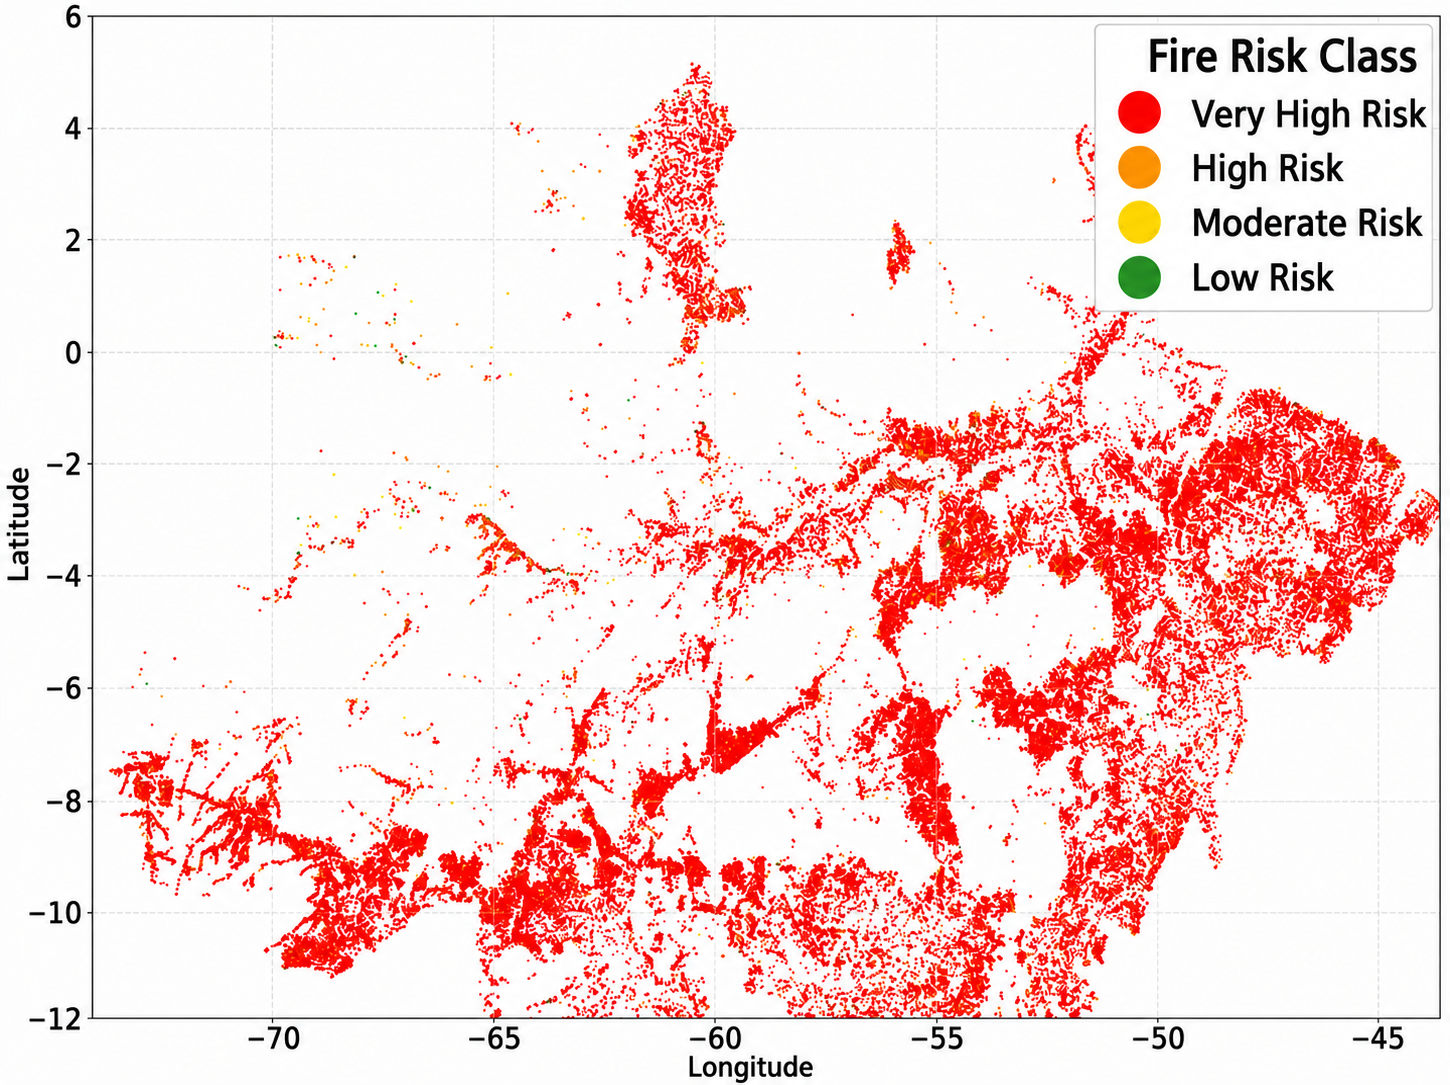
\includegraphics[width=\columnwidth]{fig2_dataset_samples.png}
  \caption{Spatial distribution of the 200,000-sample Amazon fire dataset coloured by LightGBM risk class.}
  \label{fig:dataset}
\end{figure}

\begin{table}[p]
\caption{\textbf{Feature set of the Amazon fire susceptibility dataset.}}
\label{tab:dataset}
\centering
\renewcommand{\arraystretch}{1.2}
\begin{tabularx}{\columnwidth}{|X|l|l|l|}
\hline
\textbf{Feature} & \textbf{Source} & \textbf{Type} & \textbf{Mean / Range} \\
\hline
temperature\_c       & ERA5        & Continuous  & 27.4\,°C      \\
\hline
humidity\_pct        & ERA5        & Continuous  & 74.2\%        \\
\hline
precipitation\_mm    & ERA5        & Continuous  & 4.1\,mm/day   \\
\hline
wind\_speed\_ms      & ERA5        & Continuous  & 2.3\,m/s      \\
\hline
wind\_direction\_deg & ERA5        & Continuous  & 0--360°       \\
\hline
NDVI                 & Sentinel-2  & Continuous  & 0.52          \\
\hline
NBR                  & Sentinel-2  & Continuous  & 0.31          \\
\hline
LST\_celsius         & MODIS       & Continuous  & 29.8\,°C      \\
\hline
elevation\_m         & SRTM        & Continuous  & 248\,m        \\
\hline
slope\_deg           & SRTM        & Continuous  & 3.1°          \\
\hline
aspect\_deg          & SRTM        & Continuous  & 0--360°       \\
\hline
land\_cover\_group   & MapBiomas   & Categorical & 5 classes     \\
\hline
month                & INPE/ERA5   & Ordinal     & 1--12         \\
\hline
has\_satellite\_data & GEE         & Binary      & 0\,/\,1       \\
\hline
has\_terrain\_data   & SRTM        & Binary      & 0\,/\,1       \\
\hline
fire (label)         & INPE        & Binary      & 0\,/\,1       \\
\hline
\end{tabularx}
\end{table}

\begin{table}[p]
\caption{\textbf{Seven-classifier comparison on the held-out test set (40,000 samples).}}
\label{tab:models}
\centering
\renewcommand{\arraystretch}{1.2}
\begin{tabularx}{\columnwidth}{|X|c|c|c|}
\hline
\textbf{Model} & \textbf{Acc (\%)} & \textbf{F1 (\%)} & \textbf{ROC-AUC} \\
\hline
Random Forest    & 95.12 & 95.12 & 0.9857 \\
\hline
XGBoost          & 95.53 & 95.53 & 0.9874 \\
\hline
LightGBM         & 95.55 & 95.55 & 0.9874 \\
\hline
CatBoost         & 95.49 & 95.49 & 0.9871 \\
\hline
TabNet           & 95.15 & 95.15 & 0.9863 \\
\hline
ANN/MLP          & 94.36 & 94.36 & 0.9820 \\
\hline
Stacked Ensemble & 95.53 & 95.53 & 0.9876 \\
\hline
\end{tabularx}
\end{table}

\begin{figure}[p]
  \centering
  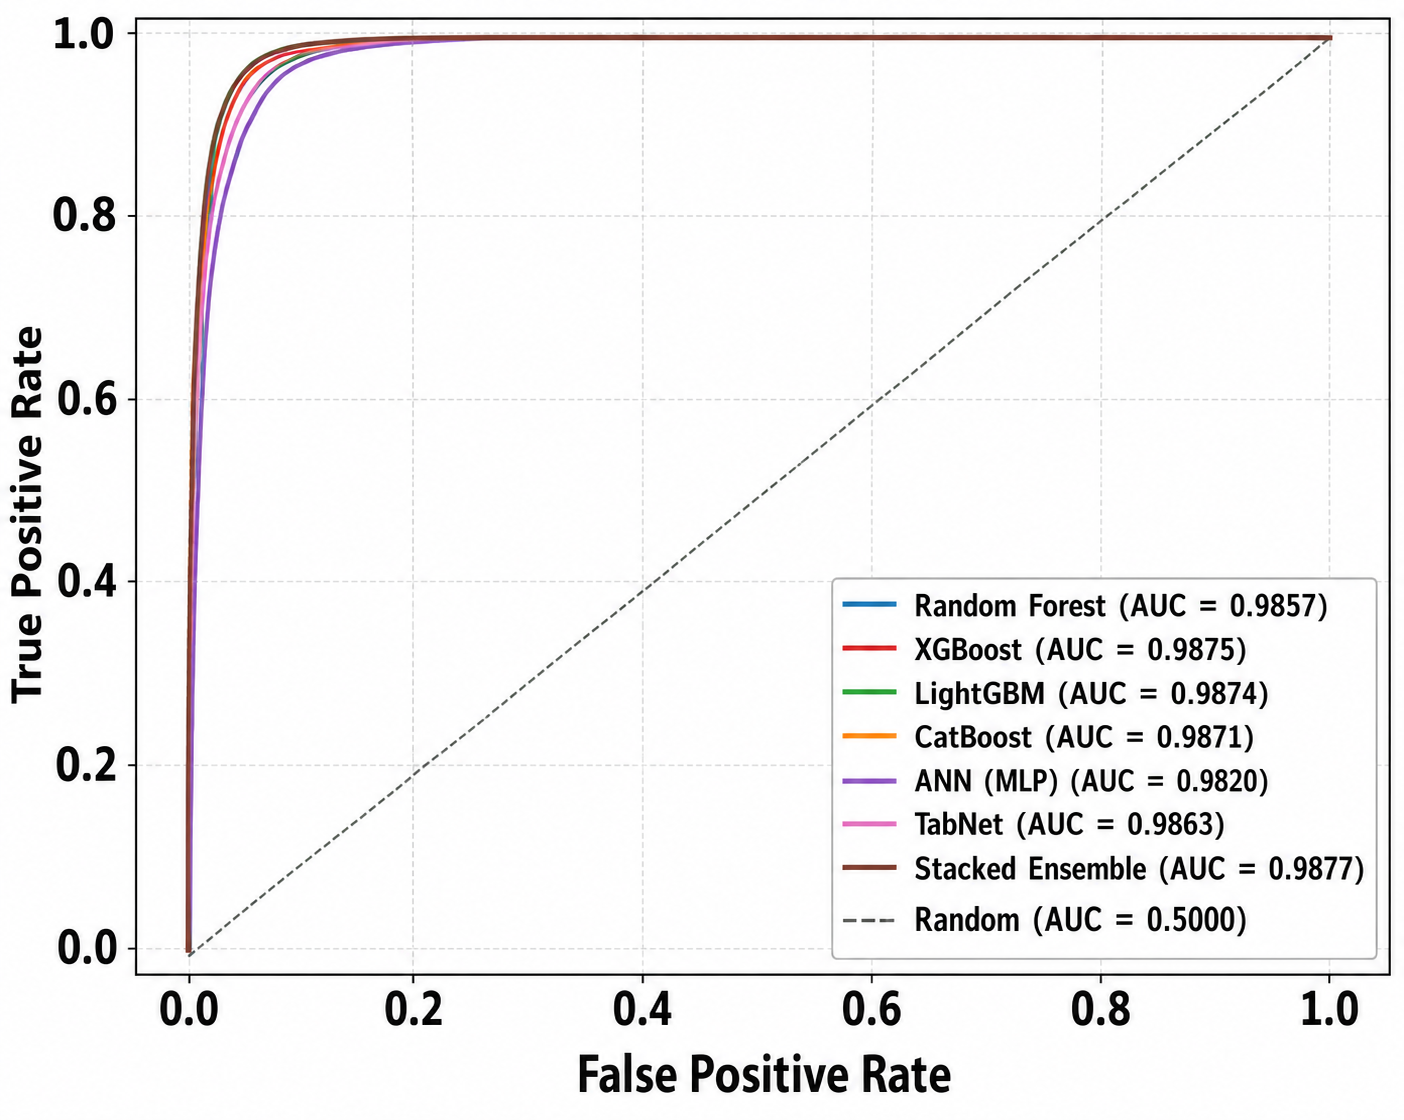
\includegraphics[width=\columnwidth]{fig4_roc_curves.png}
  \caption{ROC curves for Random Forest, XGBoost, and ANN/MLP; remaining AUC values in Table~\ref{tab:models}.}
  \label{fig:roc}
\end{figure}

\begin{figure}[p]
  \centering
  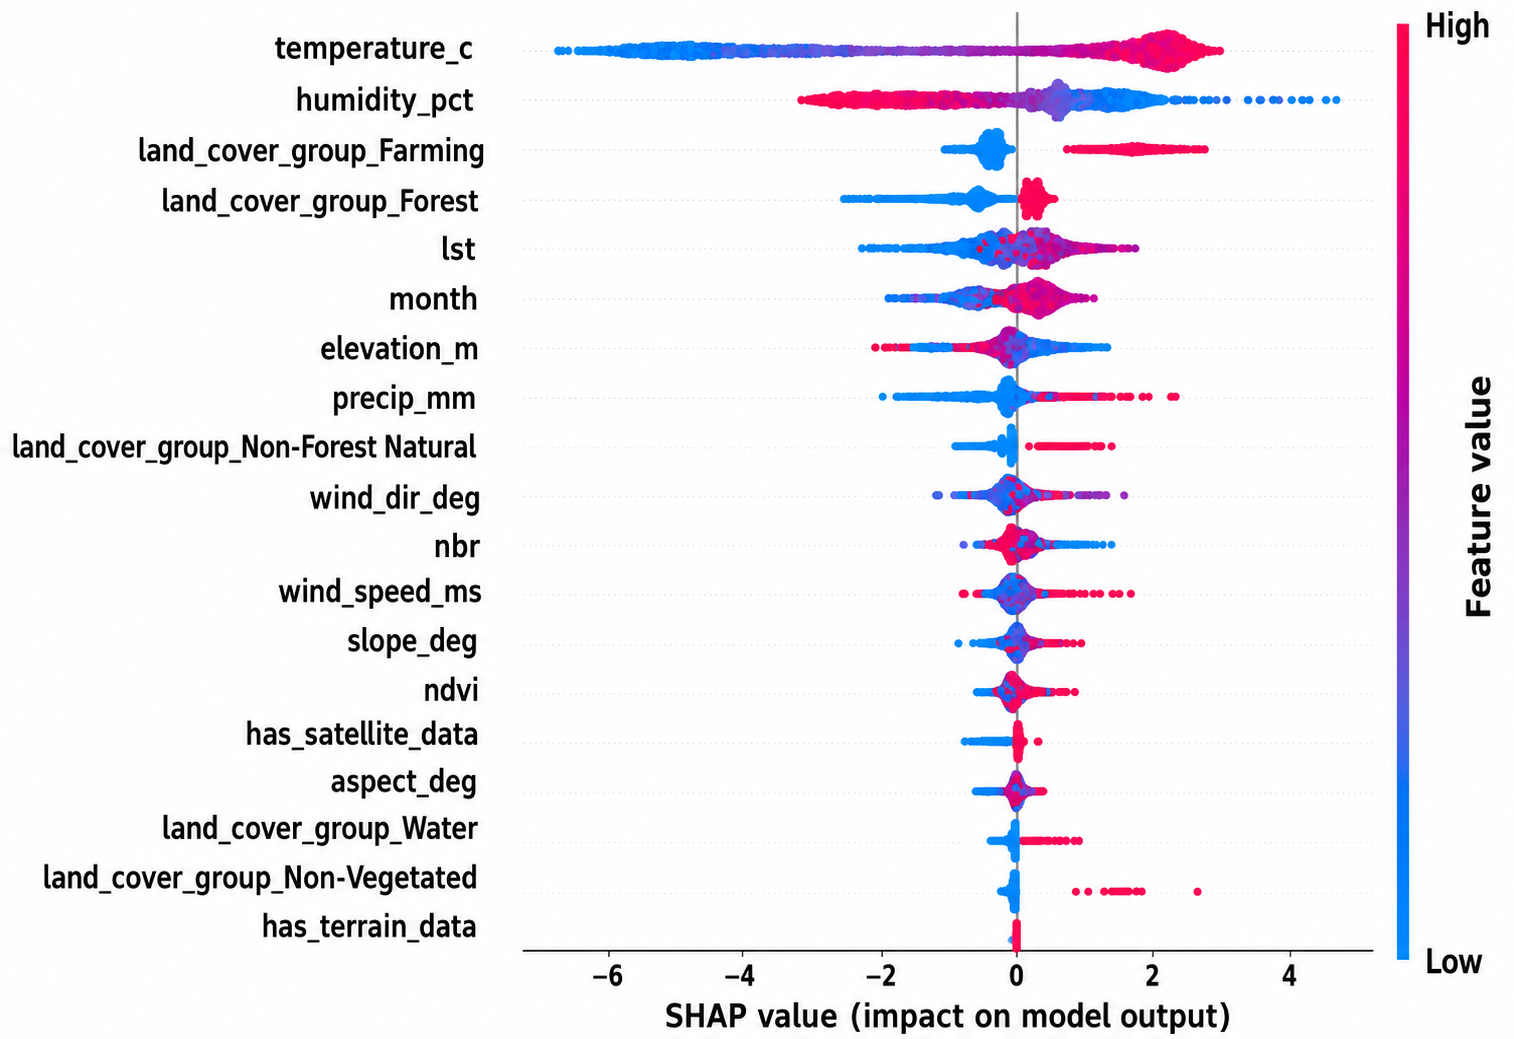
\includegraphics[width=\columnwidth]{fig5_shap_beeswarm.png}
  \caption{SHAP beeswarm summary (5,000-sample XGBoost subset), features ranked by mean $|\phi|$.}
  \label{fig:shap}
\end{figure}

\begin{figure}[p]
  \centering
  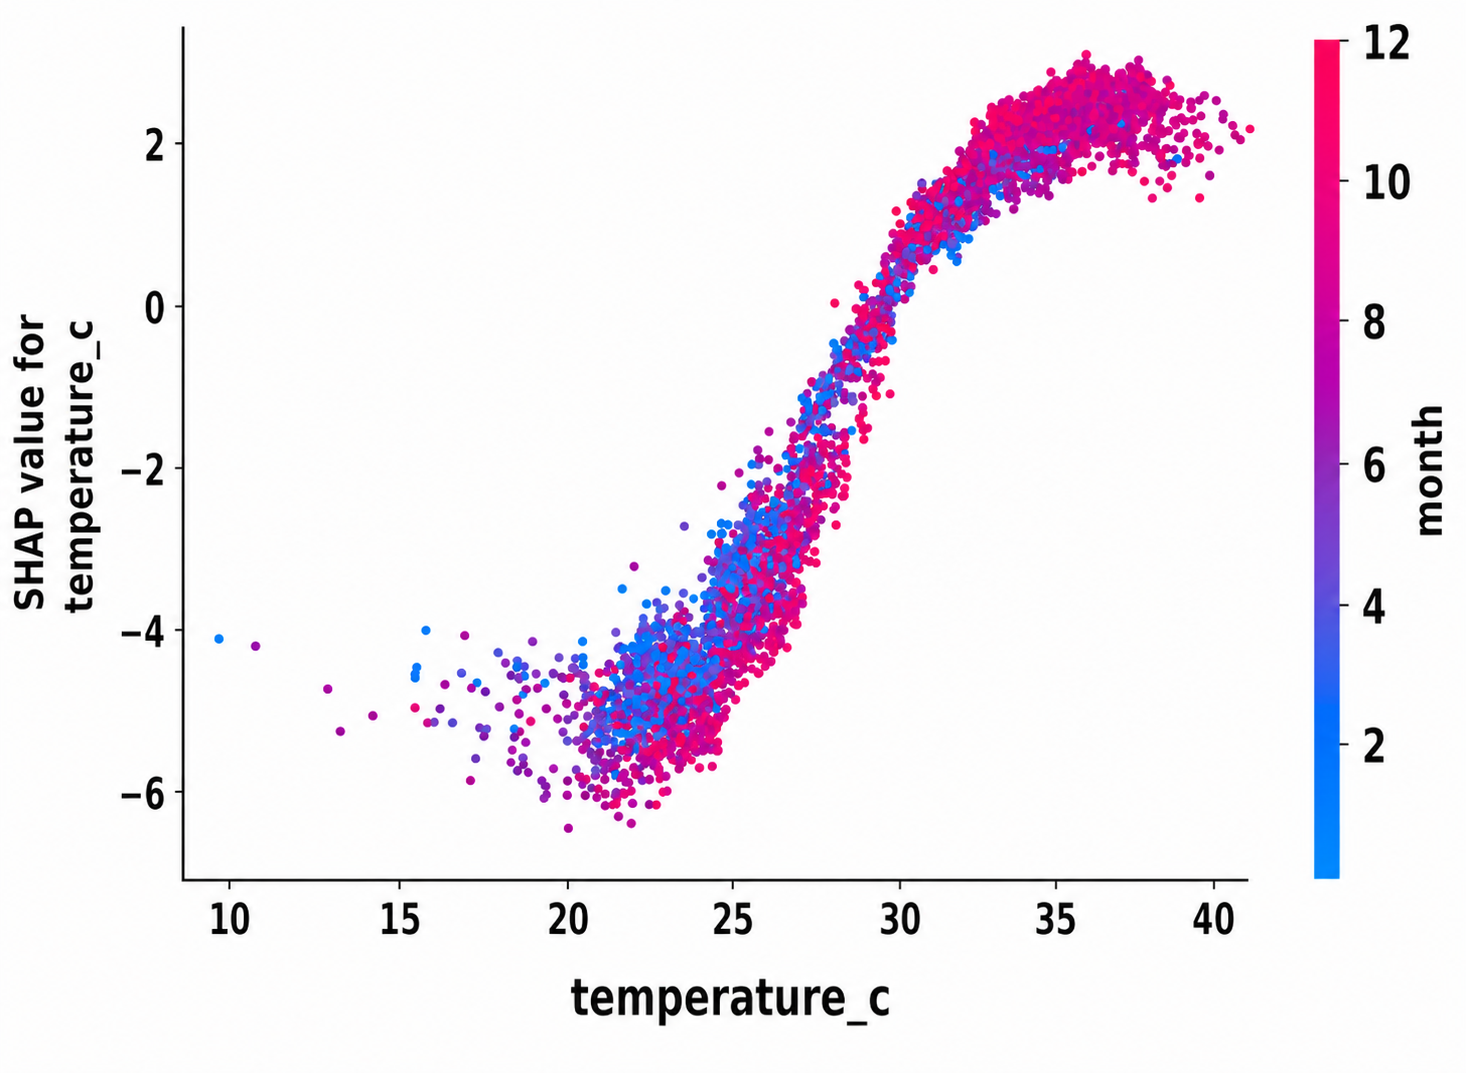
\includegraphics[width=\columnwidth]{fig6_shap_dependence.png}
  \caption{SHAP dependence plot for temperature\_c coloured by month, showing threshold behaviour above 30\,°C.}
  \label{fig:shap_dep}
\end{figure}

\begin{figure}[p]
  \centering
  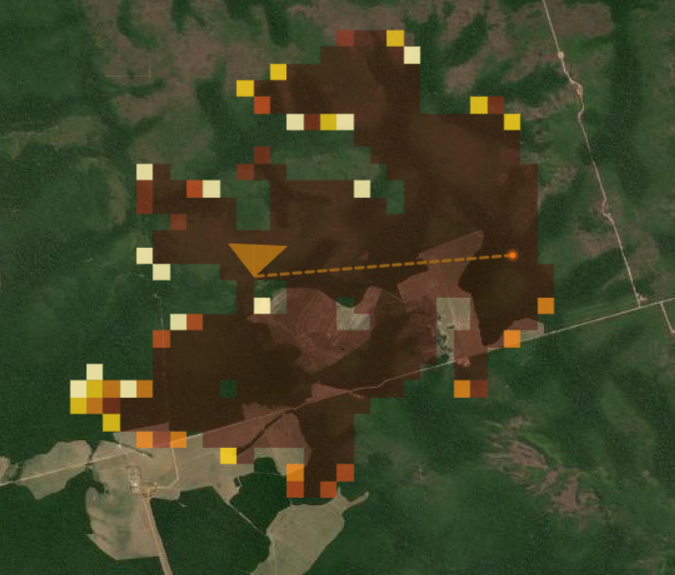
\includegraphics[width=\columnwidth]{fig7_fire_spread_map.png}
  \caption{12-hour CA burn footprint on the 51$\times$51 grid (100\,m cells), colour-coded by ignition time.}
  \label{fig:spread}
\end{figure}

\begin{figure}[p]
  \centering
  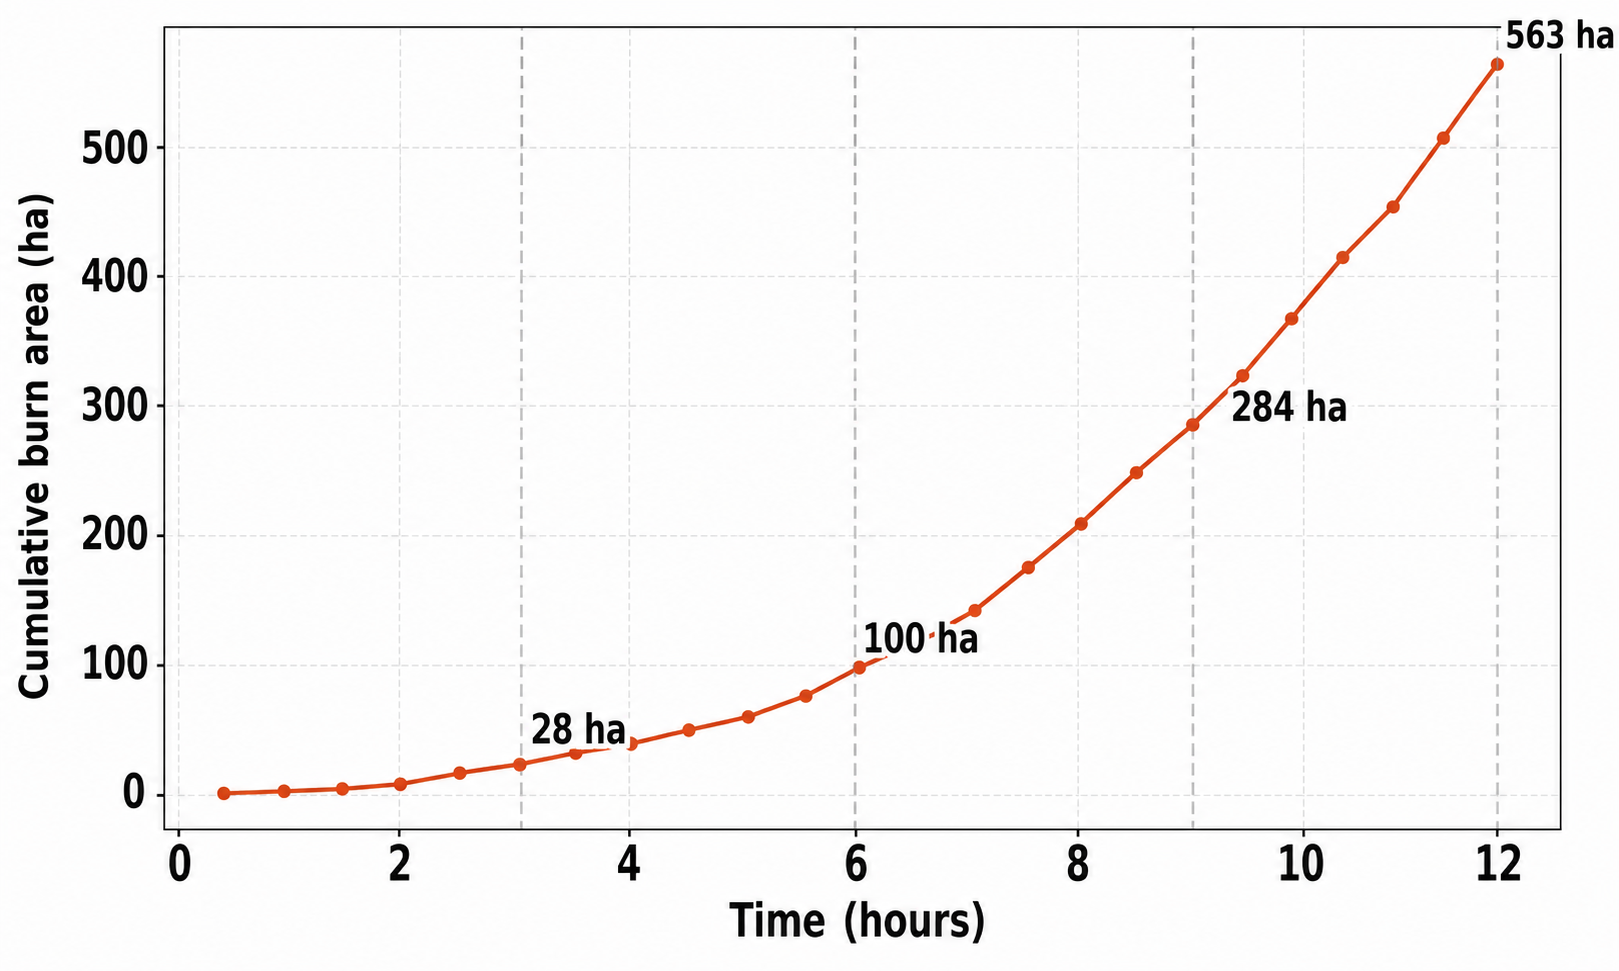
\includegraphics[width=\columnwidth]{fig8_burn_area_growth.png}
  \caption{Cumulative burn area over 12 hours: 28\,ha at 3\,h, 100\,ha at 6\,h, 284\,ha at 9\,h, 563\,ha at 12\,h.}
  \label{fig:burn_growth}
\end{figure}

\begin{table}[p]
\caption{\textbf{GIS ecological risk indices computed from live ERA5 satellite snapshot.}}
\label{tab:risk}
\centering
\renewcommand{\arraystretch}{1.2}
\begin{tabularx}{\columnwidth}{|l|l|X|l|}
\hline
\textbf{Index} & \textbf{Value} & \textbf{Entities Covered} & \textbf{Risk Band} \\
\hline
PAVI (0--10) & 1.3838 & 143 ICMBio protected areas    & Moderate \\
\hline
ITRI (0--10) & 1.1318 & 351 FUNAI indigenous territories & Moderate \\
\hline
STS (1--4)   & 1.5846 & 130 settlements (10\,km radius) & Low--Moderate \\
\hline
Mean FVI     & 3.2641 & 45,000 grid cells (100\,km$^2$) & Moderate \\
\hline
\end{tabularx}
\end{table}

\begin{figure}[p]
  \centering
  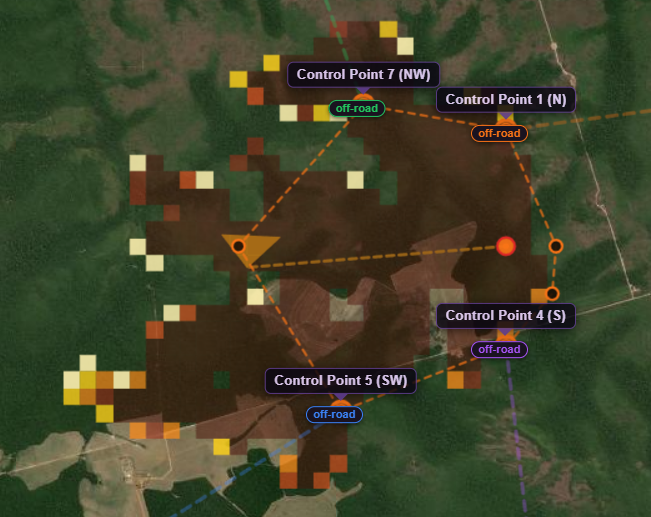
\includegraphics[width=\columnwidth]{fig9_agent_coordination.png}
  \caption{Live agent coordination output: control points placed around the fire perimeter on satellite imagery.}
  \label{fig:agent_coord}
\end{figure}

\begin{table}[p]
\caption{\textbf{Live coordination results: 2, 4 and 6 crews against 11 threatened assets.}}
\label{tab:coord_scale}
\centering
\renewcommand{\arraystretch}{1.2}
\begin{tabularx}{\columnwidth}{|c|c|X|c|c|c|}
\hline
\textbf{Crews} & \textbf{Protected} & \textbf{Area saved (ha)} & \textbf{FIP (\%)} & \textbf{Time (s)} & \textbf{Cost (\$)} \\
\hline
2 & 2\,/\,11 & 21{,}642 & 18.2 & 25.87 & 0.00466 \\
\hline
4 & 4\,/\,11 & 38{,}754 & 36.4 & 26.30 & 0.00503 \\
\hline
6 & 6\,/\,11 & 83{,}031 & 54.5 & 35.08 & 0.00645 \\
\hline
\end{tabularx}
\end{table}

\begin{table*}[p]
\caption{\textbf{Realized protected priority across 216 factorial benchmark scenarios (Wilcoxon signed-rank, Holm-corrected; $r_{\text{rb}}$ = rank-biserial).}}
\label{tab:expA}
\centering
\renewcommand{\arraystretch}{1.2}
\begin{tabularx}{\textwidth}{|l|c|c|X|c|c|}
\hline
\textbf{Comparison} & \textbf{A mean} & \textbf{B mean} & \textbf{$\Delta$ [95\% CI]} & \textbf{$p$-value} & \textbf{$r_{\text{rb}}$} \\
\hline
Stale $\to$ Ours   & 19.40 & 24.49 & $+5.09\ [4.59,\ 5.59]$ & $1.83\times10^{-27}$ & $+1.00$ \\
\hline
Ours $\to$ Oracle  & 24.49 & 24.49 & $0.00$                  & ---                  & ---     \\
\hline
Stale $\to$ Oracle & 19.40 & 24.49 & $+5.09\ [4.59,\ 5.59]$ & $1.83\times10^{-27}$ & $+1.00$ \\
\hline
\end{tabularx}
\end{table*}

\EOD

\end{document}
